%\usepackage{subcaption}
%\usepackage{sectsty}
%\allsectionsfont{\normalfont\scshape} 
%\input{tcilatex}
%\input{tcilatex}


\documentclass[superscriptaddress, notitlepage]{revtex4-1}
%%%%%%%%%%%%%%%%%%%%%%%%%%%%%%%%%%%%%%%%%%%%%%%%%%%%%%%%%%%%%%%%%%%%%%%%%%%%%%%%%%%%%%%%%%%%%%%%%%%%%%%%%%%%%%%%%%%%%%%%%%%%%%%%%%%%%%%%%%%%%%%%%%%%%%%%%%%%%%%%%%%%%%%%%%%%%%%%%%%%%%%%%%%%%%%%%%%%%%%%%%%%%%%%%%%%%%%%%%%%%%%%%%%%%%%%%%%%%%%%%%%%%%%%%%%%
\usepackage[T1]{fontenc}
\usepackage[english]{babel}
\usepackage{amsmath,amsfonts,amsthm}
\usepackage{graphicx}
\usepackage{booktabs}
\usepackage{xcolor}
\usepackage{pgfplots}
\usepackage{anyfontsize}
\usepackage{calc}
\usepackage{tikz}
\usepackage{braket}
\usepackage{lipsum}
\usepackage{wrapfig}
\usepackage[margin=0.75in]{geometry}
\usepackage{pdfpages}
\usepackage{fancyhdr}
	
\usepackage{chngcntr}
 
\counterwithout{figure}{section}
\counterwithout{table}{section}
%\usepackage[style=numeric,sorting=none]{biblatex}

\setcounter{MaxMatrixCols}{10}
%TCIDATA{OutputFilter=LATEX.DLL}
%TCIDATA{Version=5.50.0.2953}
%TCIDATA{<META NAME="SaveForMode" CONTENT="1">}
%TCIDATA{BibliographyScheme=Manual}
%TCIDATA{LastRevised=Tuesday, October 30, 2018 17:31:48}
%TCIDATA{<META NAME="GraphicsSave" CONTENT="32">}

\makeatletter
\AtBeginDocument{\let\LS@rot\@undefined}
\makeatother
\pgfplotsset{compat=newest}
\usetikzlibrary{arrows}
\usetikzlibrary{calc}
\newenvironment{colvec}{\left(\begin{array}{c}}{\end{array}\right)}
\pagestyle{fancyplain} 
\fancyhead[L]{V. Premakumar} 
\fancyfoot[L]{} 
\fancyfoot[C]{} 
\fancyfoot[R]{\thepage} 
\renewcommand{\headrulewidth}{0pt} 
\renewcommand{\footrulewidth}{0pt} 
\renewcommand{\vec}[1]{\mathbf{#1}}
\newcommand{\npder}[3]{\frac{\partial^{#3} #1}{\partial #2^{#3}}}
\setlength{\headheight}{13.6pt} 
\newcommand{\E}{\mathcal{E}}
\newcommand{\pder}[2]{\frac{\partial #1}{\partial #2}}
%\numberwithin{equation}{section} 
%\numberwithin{figure}{section} 
%\numberwithin{table}{section} 
\DeclareMathOperator{\sech}{sech}
\DeclareMathOperator{\csch}{csch}
\DeclareMathOperator{\arcsec}{arcsec}
\DeclareMathOperator{\arccot}{arcCot}
\DeclareMathOperator{\arccsc}{arcCsc}
\DeclareMathOperator{\arccosh}{arcCosh}
\DeclareMathOperator{\arcsinh}{arcsinh}
\DeclareMathOperator{\arctanh}{arctanh}
\DeclareMathOperator{\arcsech}{arcsech}
\DeclareMathOperator{\arccsch}{arcCsch}
\DeclareMathOperator{\arccoth}{arcCoth}
\DeclareMathOperator{\Span}{span}
\DeclareMathOperator{\Tr}{Tr}
%\setlength\parindent{0pt} 
\newcommand{\horrule}[1]{\rule{\linewidth}{#1}}
%\input{tcilatex}

%\addbibresource{bibliography.bib}

\begin{document}


\title{Supplemental Material for 2-designs and Redundant Syndrome Extraction for Quantum Error Correction }
\author{Vickram N. Premakumar}
\address{Physics Department, University of Wisconsin-Madison, 1150 Univ. Ave., Madison, WI, USA}
\author{Hele Sha}
\address{Physics Department, University of Wisconsin-Madison, 1150 Univ. Ave., Madison, WI, USA}
\author{Daniel Crow}
\address{Physics Department, University of Wisconsin-Madison, 1150 Univ. Ave., Madison, WI, USA}
\author{Eric Bach}
\address{Computer Science Department, University of Wisconsin-Madison, Madison, WI, USA}
\author{Robert Joynt}
\address{Physics Department, University of Wisconsin-Madison, 1150 Univ. Ave., Madison, WI, USA}
\address{
	Kavli Institute for Theoretical Sciences, University of Chinese Academy of Sciences, Beijing 100190, China}
\date{{\normalsize \today}}

\maketitle

\section{Constraints on BIBD Parameters for QEC}

\subsection{Proof of constraint 1}
We must show that all the measured stabilizers $S$ commute with all the logical operators $L$ if and only if $w$ is even.
An example of such a commutator is 
\begin{equation*}
[S,L] = [ Z_{i_1} Z_{i_2} ... Z_{i_w}, X_1 X_2... X_n ],
\end{equation*}
where $ \{i_1,i_2,...i_w \} \subset  \{1,2,...,n\}$.  We then define the set of indices $\{k_1,k_2...k_{(n-w)} \}$ such that 
$ \{i_1,i_2,...i_w \} \cup \{j_1,j_2...j_{(n-w)} \} = \{1,2...n\}$
This can be simplified as follows: 
\begin{eqnarray*}
	[S,L] 
	& = & [Z_{i_1} Z_{i_2} ... Z_{i_w}, X_1 X_2... X_n] \\
	& = & X_{k_1} X_{k_2}... X_{k_{(n-w)}} [Z_{i_1} Z_{i_2} ... Z_{i_w}, X_{i_1} X_{i_2}... X_{i_w}] \\
	& = &  X_{k_1} X_{k_2}... X_{k_{(n-w)}}  \times \\
	&  &  (Z_{i_1} Z_{i_2} ... Z_{i_w}X_{i_1} X_{i_2}... X_{i_w} -  X_{i_1} X_{i_2}... X_{i_w} Z_{i_1} Z_{i_2} ... Z_{i_w}) \\
	& = &  X_{k_1} X_{k_2}... X_{k_{(n-w)}} \times \\
	& &  (Z_{i_1} X_{i_1} Z_{i_2} X_{i_2} ... Z_{i_w}X_{i_w} -  X_{i_1} Z_{i_1} X_{i_2} Z_{i_2}... X_{i_w} Z_{i_w}) \\
	& = &  X_{k_1} X_{k_2}... X_{k_{(n-w)}} \times \\
	& &  ((-1)^w X_{i_1} Z_{i_1} X_{i_2} Z_{i_2} ... X_{i_w}Z_{i_w} -  X_{i_1} Z_{i_1} X_{i_2} Z_{i_2}... X_{i_w} Z_{i_w}) \\
	& = &  X_{k_1} X_{k_2}... X_{k_{(n-w)}} [ (-1)^w -1] X_{i_1} Z_{i_1} X_{i_2} Z_{i_2} ... X_{i_w}Z_{i_w},
\end{eqnarray*}
which is zero if and only if $w$ is even.  This proof clearly holds for all stabilizer/logical operator pairs.

\subsection{Proof of constraint 2}
For the CSS-DBR codes, the same design is used twice, once for the X-stabilizers and once for the Z-stabilizers.  The full group must be abelian, so one must check that the X-stabilizers commute with the Z-stabilizers. The relevant commutators have the form 
\begin{equation*}
C =  [ X_{i_1} X_{i_2} ... X_{i_w} , Z_{j_1} Z_{j_2} ... Z_{j_w} ] 
\end{equation*}
Here $ \{i_1,i_2,...i_w \} \subset  \{1,2,...,n\}$. and $ \{j_1,j_2,...j_w \} \subset  \{1,2,...,n\}$. Inspection of the proof for constraint 1 then indicates that if we define 
\begin{equation*}
x = | \{i_1,i_2,...i_w \} \cap \{j_1,j_2,...j_w \} |,
\end{equation*}
then $C=0$ if and only if $x$ is even.  This is true for all choices of the index sets if $\lambda$ is even.   

\section{Failure Rates}

In the main text we showed the failure rates of traditional QEC compared with two proposed extensions by plotting the difference as a function of both physical and measurement error rates. To emphasize the region of interest for near-threshold quantum computers, we restricted $p_q, p_m$ to a small range close to zero. For completeness, we include the full comparison over the entire feasible parameter range. When the curve where $F_{QEC} - F_{MR/DBR} = 0$ does not pass through the origin, this reflects a difference in the power of the leading order $p_q$ or $p_m$ between the two rates. That is to say, one method can tolerate more errors of a certain type than the other when this is the case.

\begin{figure}
	\centering
	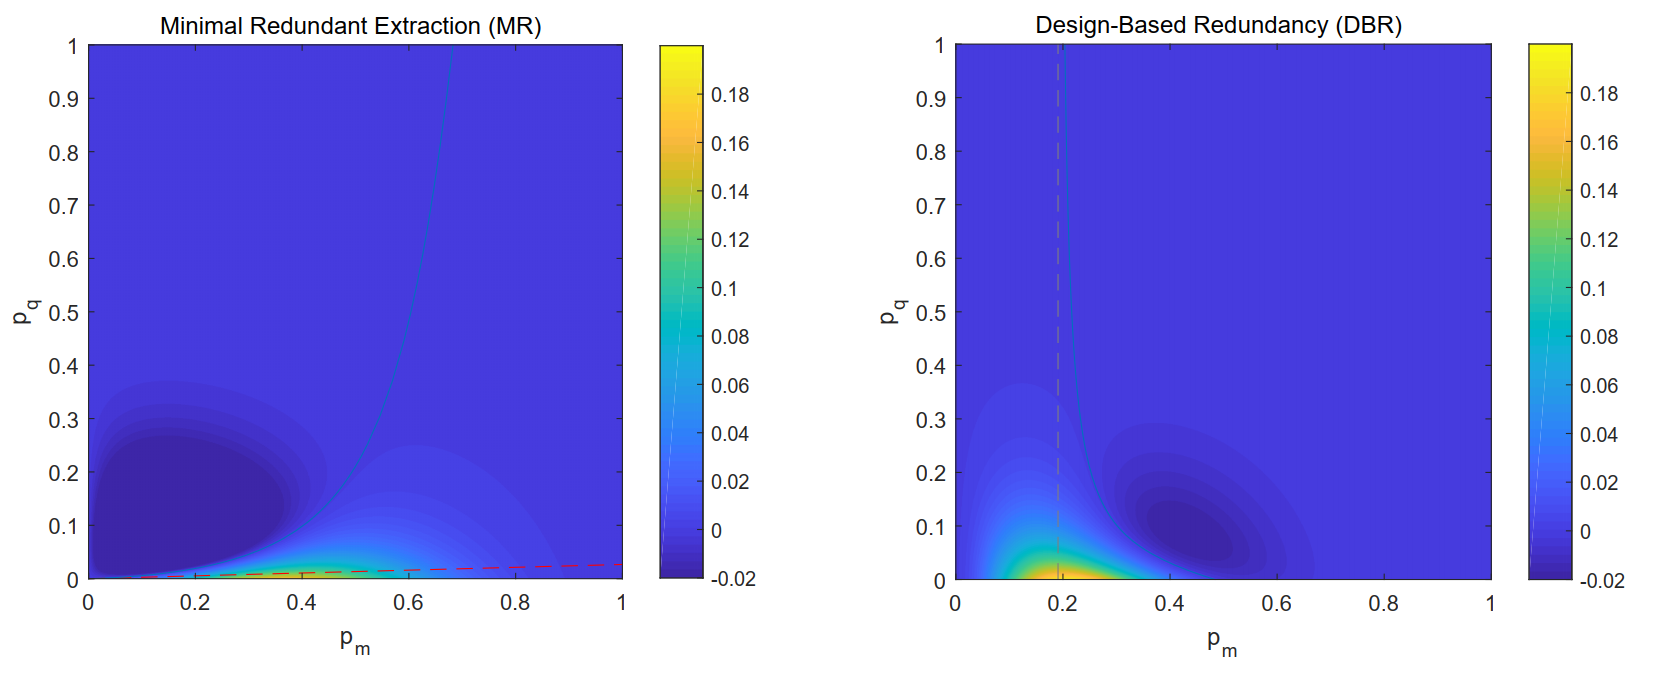
\includegraphics[width=\linewidth]{5_qubit_crop.png}
	\caption{$F_{QEC} - F_{MR}$ and $F_{QEC} - F_{DBR}$ for the [[5,1,3]] Perfect code. This is a zoomed-out version of the plot in the main text showing the results for all possible error rates.}
	\label{fig:5qubitperfectcodefullrange}
\end{figure}

\begin{figure}
	\centering
	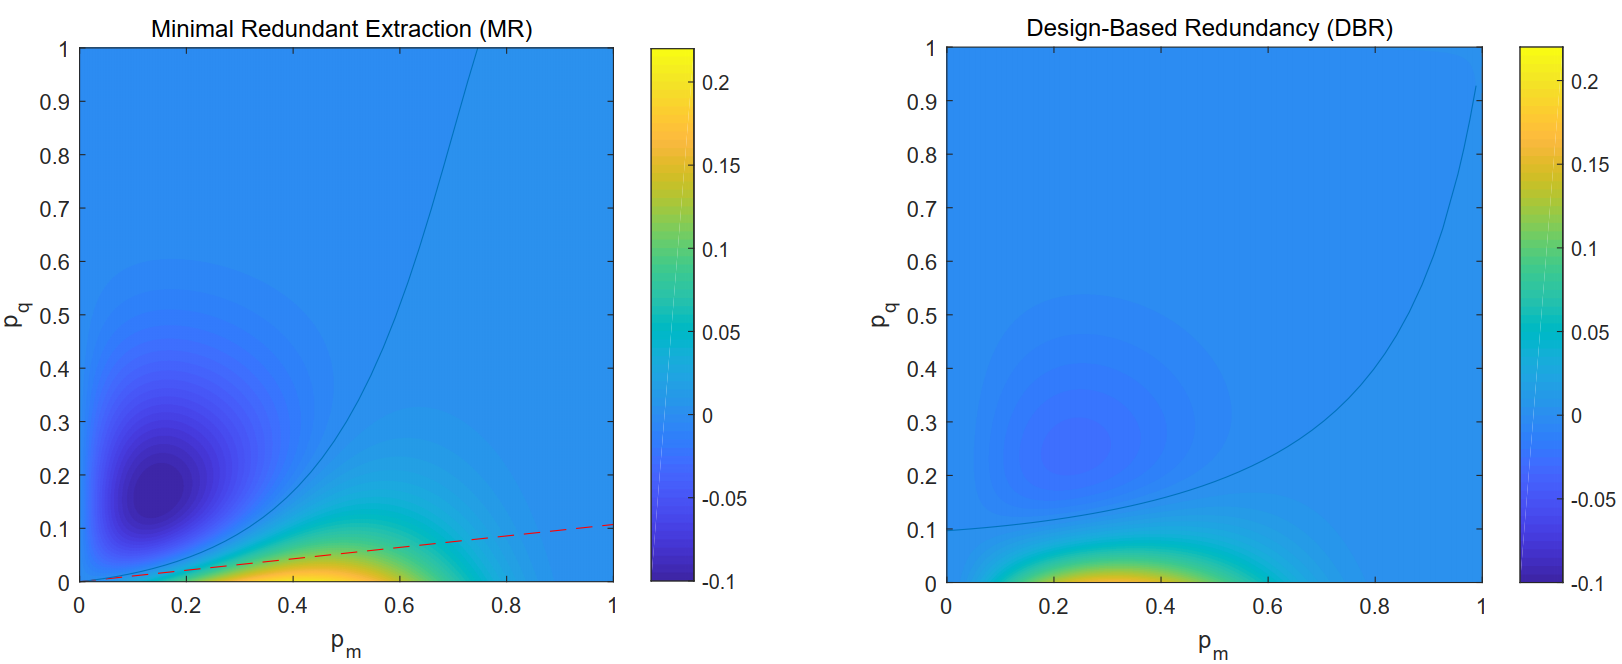
\includegraphics[width=\linewidth]{steane_crop.png}
	\caption{$F_{QEC} - F_{MR}$ and $F_{QEC} - F_{DBR}$ for the [[7,1,3]] Steane code. This is a zoomed-out version of the plot in the main text showing the results for all possible error rates.}
	\label{fig:steanecodefullrange}
\end{figure}

We also provided truncated analytic forms for the failure rates as a function of $p_q, p_m$, here we include the full expressions.



\end{document}
